\section{Introduction}\label{sec_introduction}

Given data from two related tasks, how much does combining both data for learning a joint model help predict one of the tasks of interest?
For example, suppose you have $n_1$ datapoints with $p$-dimensional covariates (sampled from a distribution $D_1$) and real-valued labels in the first task, and $n_2$ datapoints with $p$-dimensional covariates (sampled from a different distribution $D_2$) and real-valued labels in the second task. 
Does combining the $n_1 + n_2$ datapoints help learn a model whose performance is better than a model learned using the $n_2$ datapoints alone?
Such questions are prevalent in transfer learning, where one often uses data from related tasks to expand the sample size of a task of interest.
A frequent impediment to applying transfer learning is \textit{negative information transfer} if combining both data performs worse than learning a single task clone \cite{PY09}.
\textit{Positive information transfer} refers to the desirable scenario where a task of interest benefits when combined with another task.

The answer to the two questions above hinges on the tasks' heterogeneity.
For example, negative information transfer can happen if the label distribution of the second task conditional on the covariates deviates significantly from that of the first task.
Additionally, the ``information transfer effect'' also hinges on the covariates' distributions, $D_1$ and $D_2$.
Following the existing literature (e.g., \citet{kouw2018introduction}), we refer to settings where $D_1 \neq D_2$ as \textit{covariate shift} and settings where label distributions differ (conditional on the covariates) as \textit{model shift}.
Both covariate and model shifts are prevalent in modern datasets (see e.g., \citet{koh2021wilds}).

This paper studies a linear regression setting involving two tasks with covariate and model shifts.
We use a two-layer linear neural network to combine the data from both tasks and show that this network reproduces several interesting phenomena in transfer learning.
We analyze the prediction risk of this network and its transfer effect, providing precise conditions based on geometries of $D_1, D_2$, and the sample sizes $n_1, n_2$.
The analysis has also inspired several insights for understanding and mitigating covariate and model shifts.

The key ingredient of our analysis is showing the asymptotic limit of certain combinations of sample covariance matrices under distribution shift, using the local laws developed recently by \citet{isotropic} and \citet{BES_free1}.
After formally defining the specific problem that we tackle, in Section \ref{sec_related}, we provide a technical discussion of the related works in random matrix theory.

%Our main contribution is to precisely analyze a number of interesting phenomena including the above that are prevalent in transfer learning, depending on .
 %an analysis of the precise causes of negative transfer is of significant practical interest.

\subsection{Setup and motivating examples}\label{sec_mot}

Let $i = 1$ or $2$.
Let $x_1^{(i)}, x_2^{\ss (i)}, \dots, x_{n_i}^{(i)}$ be the covariates.
Let $y_1^{(i)}, y_2^{(i)}, \dots, y_{n_i}^{(i)}$ be the corresponding labels.
We assume a linear model specified by an unknown model vector $\beta^{(i)} \in \real^p$ as follows:
\begin{align}
    y_j^{(i)} = \inner{x_j^{(i)}}{\beta^{(i)}} + \varepsilon_j^{(i)}, \text{ for any } j = 1,\dots,n_i, \label{eq_linear}
\end{align}
where $\varepsilon^{(i)}_j\in\real$ denotes a random noise variable with mean zero and variance $\sigma^2$.
For the ease of presentation, we refer to the first dataset as the source and the second task as the target.
%Our goal is to learn an estimator to predict the target task given both datasets.

We learn a two-layer linear neural network with parameters $A \in \real^{p\times r}$, $B_1 \in \real^{r}$, and $B_2 \in \real^r$ by minimizing the following optimization objective:
\begin{align}\label{eq_hps}
    f(A, B_1, B_2) = \bignorm{X^{(1)} A B_1 - Y^{(1)}}_2^2 + \bignorm{X^{(2)} A B_2 - Y^{(2)}}_2^2.
\end{align}
The above objective uses $A$ as the shared feature space for both tasks and $B_1, B_2$ as the prediction head for each task.\footnote{Popular variants of the objective function \eqref{eq_hps} include adding a weight parameter to each summand and adding ridge regularization. We focus on the unweighted and unregularized objective for simplicity. All of the asymptotic limits we show below can be straightforwardly extended to weighted and regularized objectives.}
Such models are also known as \textit{hard parameter sharing} \cite{C97,R17}.
We focus on the case of $r = 1$---otherwise, the global minimizer of $f(A, B_1, B_2)$ reduces to learning each task alone, resulting in no transfer effect (cf. Proposition \ref{prop_large_r} in Section \ref{sec_risk}).
In this case, let $(\hat{A}, \hat{B}_1, \hat{B}_2)$ be a global minimizer of $f(\cdot)$.
The hard parameter sharing (HPS) estimator for the target task is defined as $\hat{\beta}_2^{\MTL} \define \hat{B} \hat{A}_2$.
In order to evaluate the estimator, we will study the excess risk, which is the prediction risk at an unseen datapoint (of task two) minus $\sigma^2$, denoted as $L(\hat{\beta}_2^{\MTL})$.

As a motivating example of the above setup, we show an intriguing simulation where combining both datasets results in different transfer effects.
Figure \ref{fig_motivation} illustrates a setting where $X_1, X_2$ are sampled from an isotropic Gaussian and $\beta_1,\beta_2$ are generated so that $\norm{\beta^{(1)} - \beta^{(2)}}^2 \approx 2\mu^2$.
We observe that for $\mu = 0.25$, the transfer effect is always positive---$L(\hat{\beta}_2^{\MTL})$ is always smaller than the excess risk of OLS.
For $\mu = 0.3$ or $0.35$, the transfer effect is positive only for a restricted range of $n_1$.
On the other hand, for $\mu = 0.45$, the transfer effect is always negative.  
Our result below will imply the exact conditions for positive information transfer, depending on $\mu$ and $n_1$.

\begin{figure*}
    \centering
    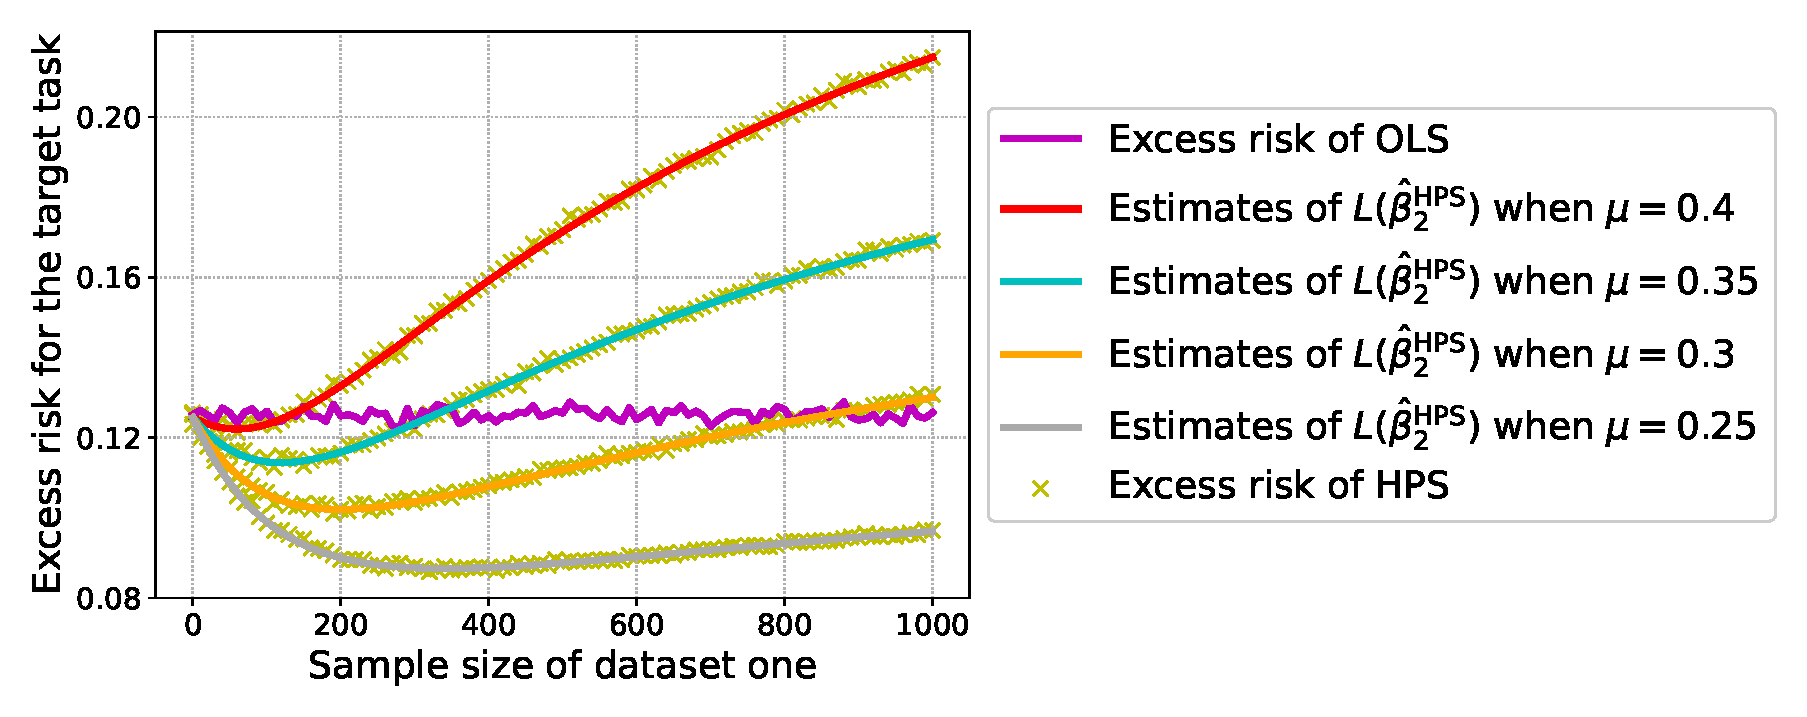
\includegraphics[width=0.8\textwidth]{figures/motivation.eps}
    \caption{We illustrate that our setup can reproduce the phenomenon of \textit{positive} (or \textit{negative}) \textit{information transfer}, which is prevalent in transfer learning.
    We vary the sample size of dataset one and the distance parameter $\mu$ such that $\norm{\beta^{(1)} - \beta^{(2)}}^2 \approx 2\mu^2$. The region below the excess risk of the ordinary least squares (OLS) estimator corresponds to \textit{positive information transfer}. This simulation uses $p = 100, n_2 = 300, \sigma = 1/2$. See also Figure \ref{fig_ab_data} for a similar phenomenon observed in text classification tasks.}
    \label{fig_motivation}
\end{figure*}
% when $L(\hat{\beta}_2^{\MTL})$ is smaller than the excess risk of the OLS estimator

\subsection{Summary of results}

We consider a high-dimensional setting on each dataset where the sample size $n_i$ increases with $p$ to infinity proportionally by a constant factor, which has recently received lots of interests (see e.g., \citet{hastie2019surprises} and Section \ref{sec_related} for more references).
Let $\Sigma^{(i)} \in \real^{p\times p}$ be a deterministic positive semidefinite matrix.
The covariates are assumed to have population covariance equal to $\Sigma^{(i)}$: $x_j^{(i)} = \big(\Sigma^{(i)}\big)^{1/2} z_{j}^{(i)},$ for any $j = 1,\dots,n_i,$
where $z_j^{(i)}$ consists of independent and identical entries sampled from a distribution that has zero mean, unit variance, and satisfies certain bounded moment condition (see Section \ref{sec_data} for the precise assumptions).

\paragraph{Main results.} We focus on the so called \textit{underparametrized} setting for the target task where $n_2 > p$ whereas for dataset one $n_1$ can be either smaller or greater than $p$.
Thus, the OLS estimator exists and it is well-known that the limit of its excess risk when $p$ approaches infinity is equal to $\frac{\sigma^2 p}{n_2 - p}$ (see e.g., \citet{bai2009spectral}).
By contrast, showing the asymptotic limit of $L(\hat{\beta}^{\MTL}_2)$ in the high-dimensional setting requires dealing with the inverse of the sum of two sample covariance matrices under distribution shift.
%The first challenge is dealing with \textit{covariate shift}---when $\Sigma^{(1)}$ and $\Sigma^{(2)}$ are different.
%The second challenge is dealing with \textit{model shift}---when $\beta^{(1)}$ and $\beta^{(2)}$ are different.
Our main result addresses both challenges by \todo{illustrate}.
\begin{itemize}
    \item %\textbf{Covariate shift:}
    Our first result applies to settings where $\Sigma^{(1)}$ and $\Sigma^{(2)}$ can be arbitrarily different but $\beta^{(1)} = \beta^{(2)}$.
    In Theorem \ref{thm_main_RMT}, we characterize the asymptotic limit of $L(\hat{\beta}_2^{\MTL})$ as a function of the singular values of the matrix $\big(\Sigma^{(1)}\big)^{1/2}\big(\Sigma^{(2)}\big)^{-1/2}$ and the sample sizes $n_1, n_2$.
    \item %\textbf{Model shift:}
    Our second result applies to settings where $\beta^{(1)}$ and $\beta^{(2)}$ can be arbitrarily different but $\Sigma^{(1)} = \Sigma^{(2)}$.
    In Theorem \ref{cor_MTL_loss}, we provide the asymptotic limit of $L(\hat{\beta}_2^{\MTL})$ as a function of the $\ell_2$ distance between $\beta^{(1)}$ and $\beta^{(2)}$, and the sample sizes $n_1, n_2$.
    \item %\textbf{Covariate and model shift:}
    Our third result applies to settings where both the covariance matrices and the model vectors are different between the two tasks.
    In Theorem \ref{???}, we show that when $\Sigma^{(2)}$ is isotropic, the asymptotic limit of $L(\hat{\beta}_2^{\MTL})$ is characterized by the singular values of $\Sigma^{(1)}$, the $\ell_2$ distance between $\beta^{(1)}$ and $\beta^{(2)}$), and the sample sizes $n_1, n_2$.
    Next, in Theorem \ref{prop_main_RMT}, we consider the most general setting concerning an arbitrary $\Sigma^{(2)}$. We identify an estimate of $L(\hat{\beta}_2^{\MTL})$ that becomes more and more accurate as $n_1 / n_2$ increases.
\end{itemize}

\noindent\textit{Extension to multiple sources.}
We also extend our setup to the case of having multiple data sources.
We consider a setting where all datasets have the same features but different labels, which is also known as multi-label prediction \cite{hsu2009multi}.
We show the asymptotic limit of $L(\hat{\beta}_i^{\MTL})$ under model shift (cf. Theorem \ref{thm_many_tasks}) and use the result to illustrate how to select the hidden width $r$ of $B$.

\paragraph{Theoretical insights and empirical implications.} Next, we demonstrate the power of these precise asymptotics by explaining several empirical phenomena in transfer learning.
We consider a random-effect model where $\beta^{(i)}$ is equal to a shared model vector plus per-task variances (cf. \citet{dobriban2018high}).
Under this model, we show the following \textit{theoretical insights}.
\begin{enumerate}
    \item[i)] \textit{Whether or not covariate shift helps depends on sample sizes:} We consider the covariate shift setting and show that (cf. Proposition \ref{claim_dichotomy}) when $n_1 < n_2$, transferring from a data source with $\Sigma^{(1)} \neq \Sigma^{(2)}$ can achieve a smaller $L(\hat{\beta}_2^{\MTL})$ compared to transferring from a data source with $\Sigma^{(1)} = \Sigma^{(2)}$. When $n_1 > n_2$, transferring from from a data source with $\Sigma^{(1)} \neq \Sigma^{(2)}$ always results in higher $L(\hat{\beta}_2^{\MTL})$ than transferring from a data source with $\Sigma^{(1)} = \Sigma^{(2)}$.
    \item[ii)] \textit{Identical covariance provides approximately optimal transfer under imbalanced sizes:} Additionally, in Proposition \ref{prop_covariate}, we show that when $n_1$ is greater than $n_2$ times a certain large constant factor, transferring from a data source with $\Sigma^{(1)} = \Sigma^{(2)}$ achieves an approximately minimum excess risk value, within a certain family of covariance matrices of $\Sigma^{(1)}$.
    \item[iii)] \textit{Three regimes of information transfer under model shift}: Next, we consider the model shift setting and characterize the precise range of $n_1$ under which there is a positive transfer.
    In Proposition \ref{claim_model_shift}, we show that when $\mu^2 \le \frac{\sigma^2 p}{2(n_2 - p)}$ (recall that $\norm{\beta^{(1)} - \beta^{(2)}}^2 \approx 2\mu^2$) is small, the transfer effect is positive for any $n_1$.
    When $\frac{\sigma^2 p}{2(n_2 - p)} < \mu^2 < \frac{\sigma^2 n_2}{2(n_2 - p)}$, there is a transition from positive to negative transfer, as $n_1$ increases.
    When $\frac{\sigma^2 n_2}{2(n_2 - p)} \le \mu^2$, the transfer effect is negative for any $n_1$.
    Additionally, we illustrate that these three regimes of information transfer arises under both covariate and model shift (cf. Figure \ref{fig_sec3_cov_mo_b}).
\end{enumerate}

We also complement our theoretical analysis with empirical evaluations.
As mentioned in Section \ref{sec_mot}, our motivation for studying the HPS estimator stems from its superior empirical performance for transfer learning.
We affirm that HPS indeed outperforms several commonly used estimators including weighted averages of the OLS estimators of each task (cf. \citet{bastani2020predicting}) and the ridge estimator of the target task in our setting. See Figure \ref{fig_sec51} for the result.

We then conduct a case study on six text classification tasks using HPS neural network models.
We demonstrate that our theoretical insights above imply interesting new methods for mitigating covariate shift and model shift, respectively.

First, our insight ii) above suggests the importance of mitigating covariate shift under imbalanced dataset sizes.
To this end, we consider a certain covariance alignment procedure proposed in \citet{WZR20} for mitigating covariate shift.
We show that such an alignment procedure provides more significant improvement when $n_1 / n_2$ increases.

Second, our insight iii) above suggests subsampling the source dataset under model shift.
An efficient instantiation of this above would be to increase the sample size of the source dataset gradually until performance drops.
For example, in the setting of Figure \ref{fig_motivation}, this procedure will stop right at the minimum of the local basin.
On both two-task and multi-task case studies using the six text classification datasets, such a training procedure can reduce the computational cost by $65\%$ compared to a stochastic gradient descent procedure without sacrificing accuracy.



%Our result implies that when all tasks have the same features but different labels, for any task, HPS helps reduce the task's variance compared to single-task learning but increases bias.

%\medskip
%\noindent\textbf{Proof techniques.}
%There are two main ideas in our analysis. The proof of our first result uses a geometric intuition that hard parameter sharing finds a ``rank-$r$'' approximation of the datasets.
%We carefully keep track of the concentration error between the global minimizer of $f(A, B)$ and its population version (cf. equation \eqref{eq_A_star}).
%The proof of our second result is significantly more involved because of different sample sizes and covariate shifts. We show that the inverse of the sum of two sample covariance matrices with arbitrary covariate shifts converges to a deterministic diagonal matrix asymptotically (cf. Theorem \ref{thm_main_RMT}).
%We use recently developed techniques from random matrix theory to show a sharp convergence rate.
% to obtain a sharp estimate on the..., which is commonly referred to as the \emph{local law}.
%\HZ{add several sentences on the technical insight}
%One limitation of our analysis is that in Example \ref{ex_sample_ratio}, there is an error term that can result in vacuous bounds for very small $n_1$ (cf. equation \eqref{cor_MTL_error}).
%We believe our result has provided significant initial insights, and it is an interesting question to tighten our result.
%See Section \ref{sec_conclude} for more discussions of the technical challenge.



\subsection{Related work}\label{sec_related}



\paragraph{Sample covariance matrices under distribution shift.}
In the \textit{underparametrized} setting ($n_2 > p$) which this work focuses on, when the covariates are sampled from Gaussian distributions, the precise asymptotic limit can be derived directly from properties of the Wishart distribution (see also Lemma \ref{fact_tr} and the historical notes in Section \ref{sec_bv}).
In the high-dimensional setting, the eigenvalues of Wishart matrices satisfy the well-known Marchenko–Pastur (MP) law \cite{MP}, whose Stieltjes transform characterizes the variance limit.
Furthermore, it is well-known that the MP law holds universally regardless of the underlying data distribution of the covariates \cite{bai2010spectral}. \citet{isotropic} obtained a sharp convergence rate of the empirical spectral distribution (ESD) of the MP law for sample covariance matrices with isotropic population covariance matrices. \citet{Anisotropic,DY} later extended this result to sample covariance matrices with arbitrary population covariances. These results are proved by establishing certain optimal convergence estimates of the Stieltjes transforms of sample covariance matrices, which are referred to as \emph{local laws} in the random matrix theory literature. We refer interested readers to \citet{erdos2017dynamical} and the references therein for a detailed review of related concepts.
Our technical contribution is to extend these techniques to the two-task setting and prove a local law for the sum of two sample covariance matrices with arbitrary covariate shifts.
Using the local law, we can then derive the variance limit with a precise dependence on the singular values of the covariate shift matrix $\big(\Sigma^{(1)}\big)^{1/2} \big(\Sigma^{(2)}\big)^{-1/2}$. 

%Our proof techniques use the so-called local law of random matrices, a recent development in the random matrix theory literature, called the \emph{local law} of 

%These techniques provide almost sharp convergence rates to the asymptotic limit compared to other methods such as free probability \cite{nica2006lectures}.
%We also extend the techniques in ?, which is one contribution of this work. 

%On the other hand, one may derive the asymptotic result in Theorem \ref{thm_main_RMT} with error $\oo(1)$ using the free addition of two independent random matrices in theory.

The asymptotic limit of the variance of $L(\hat{\beta}_2^{\MTL})$ (cf. equation \eqref{Lvar}) under covariate shift may also be derived using free addition in free probability theory \cite{nica2006lectures}.
However, this approach is not completely justified when the covariates are sampled from non-Gaussian distributions with non-diagonal covariate shift matrices. 
%(in the sense that it is hard to establish rigorously the free independence between two sample covariance matrices). 
Furthermore, our technique provides almost sharp convergence rates to the asymptotic limit, while it is unclear how to obtain such rates using free probability techniques, to the best of our knowledge.

The asymptotic limit of the bias of $L(\hat{\beta}_2^{\MTL})$ (cf. equation \eqref{Lbias}) involves ``asymmetric'' additions of two sample covariance matrices, whose analysis is technically involved.
Our result on the bias limit is inspired by the recent work of \citet{BES_free1,BES_free2}.
Additionally, we show a sharp convergence rate to the bias limit using free probability techniques.
Our work provides the first result in the model shift setting assuming that $\Sigma^{(1)} = \Sigma^{(2)}$ or that $\Sigma^{(2)}$ is isotropic, and the covariates are sampled from Gaussian distributions.
%To the best of our knowledge, we are not aware of any prior work on the precise bias limit in the high-dimensional setting, even for two Wishart matrices with the same population covariance matrix.
Showing the asymptotic bias limit under the most general covariate shift and model shift is an interesting open problem for future work.
See Section \ref{sec_conclude} for further discussion on the technical challenges.

\paragraph{Transfer learning theory.}
Earlier works such as \citet{B00,BS03,M06} use uniform convergence to obtain generalization bounds on transfer learning (also called domain adaptation).
The influential paper by \citet{BBCK10} proposes a rigorous model for domain adaptation in classification (see also \citet{crammer2008learning} for an earlier result).
Their main result provides a generalization bound for combining multiple data sources using an objective that averages over the risk of every datapoint.
This bound provides a principled way to reweight each data source by minimizing the bound.
From a technical perspective, uniform convergence-based techniques provide upper bounds on the excess risks.
However, analyzing the empirical phenomena of information transfer such as the ones in Figure \ref{fig_motivation} requires tight lower bounds on the excess risks.
The very recent work of \citet{mousavi2020minimax} introduced a minimax framework to quantify the fundamental limit of transfer learning.
Their result quantities the minimax risk using the distance between the source and target models.
Our work provides precise estimates that accurately match the empirical risk of commonly used estimators compared to their work.
These precise estimates are necessary for analyzing these estimators' transfer effect.

%One limitation of uniform convergence based techniques is that the results often assume that all  tasks have the same sample size, see e.g. \cite{B00,MPR16}.
%\citet{pontil2013excess}
%Moreover, these techniques do not apply to the high-dimensional setting because the results usually require a sample size of at least $p \log p$.
Finally, we discuss several concurrent works that study transfer learning in linear regression settings.
The work of \citet{li2020transfer} considers the problem of how to select useful data sources for transfer learning under model shift.
Their work provides an adaptive procedure that applies even when the set of beneficial data sources is unknown.
Our work differs from theirs in two aspects.
First, we considered a high-dimensional setting where the sample size increases with dimension proportionally by a constant factor.
We use this setting to reproduce several interesting phenomena in  transfer learning.
Second, our estimates apply even under covariate shift, whereas the result of \citet{li2020transfer} requires that there is no covariate shift between the data sources and the target task.
Another work by \citet{lei2021near} considers a  linear regression setting under distribution shift, including covariate shift and model shift.
The difference is that our setting deals with a labeled target dataset. In contrast, \citet{lei2021near} deal with an unlabeled target dataset (i.e., unsupervised domain adaptation).
%Linear models in multi-task learning have been studied in various settings, including online learning \cite{CCG10,DCSP18}, sparse regression \cite{LPTV09,LPVT11}, and representation learning \cite{BHKL19}.

%Our setting is closely related to domain adaptation \cite{DM06,BB07,BC08,DH09,MMR09,CWB11,ZS13,NB17,ZD19}.
%The important distinction is that we focus on predicting the target task using a hard parameter sharing model.
%For such models, their output dimension plays an important role of regularization \cite{KD12}.
%Below, we describe several lines of work that are most related to this work.

%Some of the earliest works on multi-task learning are Baxter , Ben-David and Schuller \cite{BS03}.
%Mauer \cite{M06} studies generalization bounds for linear separation settings of MTL.
%The benefit of learning multi-task representations has been studied for learning certain half-spaces \cite{MPR16} and sparse regression \cite{LPTV09,LPVT11}.
%Our work is closely related to Wu et al. \cite{WZR20}.
%While Wu et al. provide generalization bounds to show that adding more labeled helps learn the target task more accurately, their techniques cannot be used to explain when MTL outperforms STL.
%\todo{spell out the challenge more explicitly}

%Ando and Zhang \cite{AZ05} introduces an alternating minimization framework for learning multiple tasks.
%Argyriou et al. \cite{AEP08} present a convex algorithm which learns common sparse representations across a pool of related tasks.
%Evgeniou et al. \cite{EMP05} develop a framework for multi-task learning in the context of kernel methods.
%\cite{KD12} observed that controlling the capacity can outperform the implicit capacity control of adding regularization over $B$.
%The multi-task learning model that we have focused on uses the idea of hard parameter sharing \cite{C93,KD12,R17}.
%We believe that our theoretical framework can apply to other approaches to multi-task learning.


%One closely related work is \cite{WZR20}, which studied hard parameter sharing for two linear regression tasks.
%	\item \citet{kalan2020minimax}
%	\item \citet{lounici2011oracle}
\paragraph{Random matrix theory in machine learning.}
This work joins an emerging line of recent work that has found random matrix theory useful for studying modern machine learning techniques.
A prominent example is looking at interpolators in over-parametrized linear and logistic regression \cite{bartlett2020benign,hastie2019surprises,montanari2019generalization,liang2020just,liang2020precise}.
Interpolators can reproduce similar phenomena observed under neural networks because both models learn by ``interpolating'' the data using many parameters \cite{mei2019generalization}.
The precise rates achieved via random matrix theory can also explain the double-descent phenomenon \cite{belkin2019reconciling}.
Whereas these works deal with covariates drawn from a single distribution, our work instead tackles distribution shift given covariates sampled from two distributions. 





\subsection{Organizations}
The rest of this paper is organized as follows.
In Section \ref{sec_HPS}, we formally define the data model and describe the underlying assumptions.
We show a bias-variance decomposition of the HPS estimator, and connect the bias and variance equations to random matrix theory.
In Section \ref{sec_main}, we show precise estimates for the excess risk of the HPS estimator under covariate and model shifts.
In Section \ref{sec_exp}, we evaluate the performance of HPS estimators against several commonly used transfer learning estimators, and present two implications for migating covariate and model shift in neural networks.
In Section \ref{sec_same}, we extend our setup to transferring from multiple data sources under model shift.
Section \ref{sec_conclude} concludes the paper and discusses potential future directions.
Section \ref{app_proof_error_same_cov}, \ref{appendix RMT}, and \ref{app_iso_cov} present proofs of our results.